\section{Concentration dependence of layer thicknesses}
\label{sec:rot}

In this section, we investigate the concentration dependence of layer thickness. The average thicknesses $d$ achieved from reflection and transmission measurements are plotted against the different concentrations of the polymer solution $c$ and can be seen in figure \ref{fig:ConcReflTrans}.


\begin{figure}[ht]
    \centering
    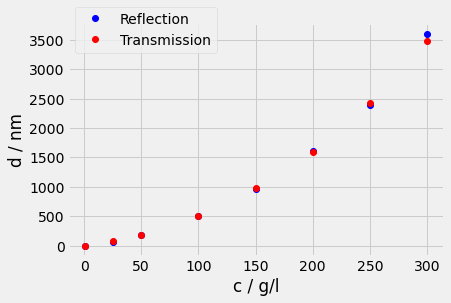
\includegraphics[width = 0.6\textwidth]{Bilder/Auswertung/Concentration/PlotReflTrans.png}
    \caption{Thickness of the films displayed as function of the concentration of the polymer solution $c$. The reflection measurements are depicted in blue, the transmission measurements in red.}
    \label{fig:ConcReflTrans}
\end{figure}

% discussion
It can be seen, that the measured thicknesses $d$ do not vary much between the reflection and transmisson measurements. In both cases $d$ increases with the concentration of the polymer in solution $c$. This is expected, as the Schubert-equation states
\begin{equation}
    d \varpropto c.
\end{equation}
In contrast, figure~\ref{fig:ConcReflTrans} does not show a linear relation between $d$ and $c$. This is due to the fact, that over the critical concentration $c^*$ the polymer chains start to overlap in the solution and the viscosity increases stronger with concentration~\cite{Ruderer.2009}. $c^*$ seperates two regimes, which can be described as two lines.

\begin{equation}
    f(c) = \Theta_1(c - c^*) \cdot (m_2c + d_{02}) - [\Theta_0(c - c^*)-1] \cdot (m_1c+d_{01})
    \label{eq:twoLines}
\end{equation}

describes a function consisting of two lines, intersecting at the critical concentration $c^*$, where $\Theta_y(x)$ is the Heaviside function with $\Theta(x=0)=y$ and $m_{1/2}$ and $d_{01/02}$ are the slopes and offset for the first/second line. \par 

The resulting fit of the data points in figure \ref{fig:ConcReflTrans} with the function $f(c)$ and parameters $c^*$, $m_1$, $m_2$, $d_{01}$ and $d_{02}$ is displayed in figure \ref{fig:FitConc}. As well in the reflection measurements as in the transmission measurements a critical conentration of \par 
\centerline{\boxed{$c$^* = \SI{150}{\milli\gram\per\milli\litre}}} \par 
is found.

\begin{figure}[ht]
    \centering
    \begin{subfigure}[b]{0.49\textwidth}
        \centering
        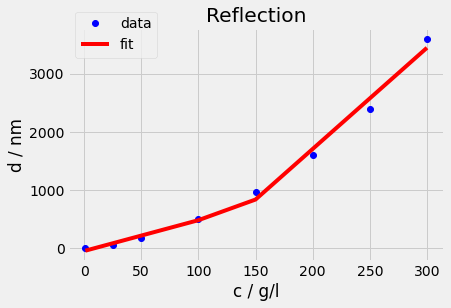
\includegraphics[width = \textwidth]{Bilder/Auswertung/Concentration/ReflFit.png}
        \caption{ }
    \end{subfigure}  
    \begin{subfigure}[b]{0.49\textwidth}
        \centering
        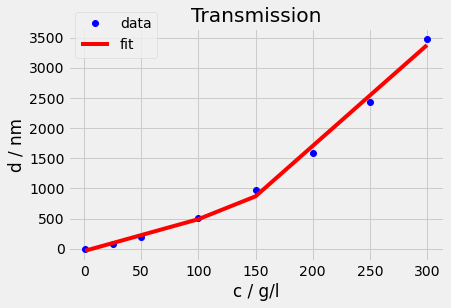
\includegraphics[width = \textwidth]{Bilder/Auswertung/Concentration/TransFit.png}
        \caption{ }
    \end{subfigure}  


    \caption{The film thickness in dependence of the concentration (blue dots) and fit using equation \ref{eq:twoLines}. As well in the reflection measurement (a) as in the transmission measuremtent (b) a critical concentration of $c^* =$ \SI{150}{\milli\gram\per\milli\litre} is found.}
    \label{fig:FitConc}
\end{figure}

The theoretical root-mean-square end-to-end distance can be calculated using 
\begin{equation}
    R_{rms} = \sqrt{C_{\infty}nL_{CC}^2} = \sqrt{2C_{\infty}m_{PS}N_AM_S^{-1}L_{CC}^2},
    \label{eq:Rrms}
\end{equation}
where $C_{\infty} = 9.5$ is the charactaristic Flory ratio for PS, $L_{CC} =$\SI{1.54}{\angstrom} is the length of a C-C-bond and the number of those bonds in the backbone of the polymer $n$ is obtained from 
\begin{equation}
    n = 2 \cdot \frac{m_{PS}}{m_S} = 2 \cdot \frac{m_{PS}N_A}{M_S}
\end{equation}
with the mass of the used PS $m_{PS} = $ \SI{35000}{\atomicmassunit}, Avogadro's constant $N_A$ and a molecular mass of the momomer styrene $M_S$ = \SI{104.15}{\gram\per\mol}~\cite{Fetters.2007,Styrol}. Using those values a root-mean-square end-to-end distance of \par
\centerline{\boxed{$R$_{rms} = \SI{123}{\angstrom}}} \par 
was obtained. \par
Another approach for calculating the root-mean-square end-to-end distance is using 
\begin{equation}
    R_{rms,exp} = 2.84 \cdot 10^{-8} \si{\mol^{-3}} \cdot (\frac{M_{PS}}{c^*})^\frac{1}{3}
    \label{eq:Daum}
\end{equation}
where $M_{PS}$ is the molecular mass of PS~\cite{Daum.1969}. This equation leads to \par 
\centerline{\boxed{$R$_{rms,exp} = \SI{175 \pm 10}{\angstrom}}} \par
Herefore, the critical concentration was being assumed to lie within \SIrange{125}{175}{\milli\gram\per\milli\litre} as the next measured concentrations from \SI{150}{\milli\gram\per\milli\litre} were \SI{100}{\milli\gram\per\milli\litre} and \SI{200}{\milli\gram\per\milli\litre}. 
%hallomats mäusssseeeeschreck, discussion why bigger
There are three common models, which describe the state of a polymer in solution: random coil, wormlike and rigid rods~\cite{Ying.1987}. For a random coil the root-mean-square end-to-end distance is given by \begin{equation}
    R_{rc} = 2 (\frac{M_{PS}}{c^*N_A})^\frac{1}{3} = 2.64 \cdot 10^{-8} \si{\mol^{-3}} \cdot (\frac{M_{PS}}{c^*})
    \label{eq:rcoil}
\end{equation}
which leads to \par 
\centerline{\boxed{$R$_{rc} = \SI{146 \pm 24}{\angstrom}.}} \par
The length of a rigid rod can be calculated as
\begin{equation}
    L_r = \sqrt{2} \cdot (\frac{M_{PS}}{c^*N_A})^\frac{1}{3} = 1.67 \cdot 10^{-8} \si{\mol^{-3}} \cdot (\frac{M_{PS}}{c^*}),
    \label{eq:rod}
\end{equation}
which leads to \par 
\centerline{\boxed{$L$_{r} = \SI{103 \pm 17}{\angstrom}.}} \par
The end-to-end distance of a wormlike structure $\widetilde{L}$ is calculated like a rigid rod. Therefore, 
\begin{equation}
    \widetilde{L} = L_r.
\end{equation} 
The model of a wormlike structure lies inbetween the random coil model and the rigid rod model regarding the rigidity of the bonds between the monomers. While in the random coil model every possible conformation can be taken independently from the other monomers, a rigid rod fixes all bounds for a maximum total length. A wormlike structure allows some flexibility, which is described by the persistance length $L_p$~\cite{Ying.1987}. Therefore, for obtaining the actual length of the chain $L_w$, the persistance length $L_p$ has to be taken in account: 
\begin{equation}
    \widetilde{L}^2 = L_w L_p
\end{equation}
$L_p$ can be calculated in the following way:
\begin{equation}
    L_p = \frac{L_k}{2} = \frac{C_{\infty}L_a}{2} = C_{\infty}L_{CC}\sin(\frac{\SI{109.5}{\degree}}{2}),
    \label{eq:Lpers}
\end{equation}
where $L_k$ is the Kuhn-length and $L_a$ is the actual end-to-end length of the polymer~\cite{Koltzenburg.2013}. The latter was calculated by assuming the backbone consisting only of C-C-bonds enclosing an angle of \SI{109.5}{\degree}. Following these equations one finds \par 
\centerline{\boxed{$L$_{w} = \SI{900 \pm 300}{\angstrom}.}} \par
First of all, it is noticeable, that equations~\ref{eq:Daum},~\ref{eq:rcoil} and~\ref{eq:rod} are similar except for different coefficients, which derive from different assumptions regarding the structure of the polymer. Interestingly, equations~\ref{eq:Daum} and~\ref{eq:rcoil} both refer to a coilish structure, but differ regardless. This could be due to differences in the assumed structure of the coils, e.g.~density. The calculated theoretical root-mean-square end-to-end distance lies inbetween the values for a random coil and a rodlike structure. This is expected, as those structurs both resemble one end of an extremum: The random coil structure assumes the single monomeres to be freely joint without any restiction regarding the folding, whilst the rodlike structure assumes the polymer to fold into a rigid line. Therefore, also the structure of the polymer used in the measurement should lie between random coil and rodlike. \par 
A useful hint is the maximum lenght of the polymer chain used. Assuming it was a rigid rod is length is calculated as 
\begin{equation}
    L_{max} = L_S N = 2 L_{CC} \sin(\frac{\SI{109.5}{\degree}}{2}) m_{PS} N_A M_S^{-1}, 
\end{equation}

where $L_S = 2 L_{CC} \sin(\frac{\SI{109.5}{\degree}}{2})$ is the lenght of the part of the backbone of a styrene monomere using the same assumptions as in equation~\ref{eq:Lpers} and $N$ is the number of monomers in the chain calculated analogous to equation~\ref{eq:Rrms}. In this way, a value of 
\begin{equation}
    L_{max} = \SI{844}{\angstrom} 
\end{equation}
is found. As this value is much bigger than the expected length assuming a rodlike structure, this possibility can be precluded. Moreover, the calculated maximum length aligns with the calculated total length for a wormlike structure, even though it has to be kept in mind, that the error of the latter is quite big. Nevertheless, the used polymer could most likely be in a wormlike structure.